\section{Green function theory}

\begin{framenologo}
  \frametitle{Green function theory}
  \tableofcontents[currentsection]
\end{framenologo}

\subsection{Introduction}

\begin{frame}
  \frametitle{Green function}
  \framesubtitle{Introduction}

  \begin{itemize}[<+->]
    \item %
    The single particle Green function may be written as:
    \begin{equation*}
      [(E+\im\eta)\ID - \HH_\kk]\G_\kk(E) = \ID
    \end{equation*}
    
    \item%
    This may be rewritten in terms of the eigenstates
    \begin{equation*}
      \G_\kk(E) = \sum_i \frac{|\psi_{i,\kk}\rangle\langle \psi_{i,\kk}|}{E+\im\eta-\E_{i,\kk}}
    \end{equation*}

    \item%
    Taking the imaginary part of the Green function yields
    \begin{align*}
      \Im \G_\kk(E) &= -\sum_i |\psi_{i,\kk}|^2\mathfrak{L}_{i,\kk}(E)
      \\
      \mathfrak{L}_{i,\kk}(E) &= \frac{\eta}{(E-\E_{i,\kk})^2 + \eta^2}
    \end{align*}
    
    \uncover<+->{
        \begin{center}
          \begin{tikzpicture}[my fill/.style={fill=good},
            font=\footnotesize]
            \begin{axis}[width=.7\textwidth,height=3.5cm,%
              xmin=-1,xmax=1,ymin=0,xlabel=Energy]
              \addplot[black,smooth,my fill] table {../data/lorentzian.dat};
              \addlegendentry{$\mathfrak{L}$}
              \draw[<->] (axis cs:-0.05, {.5/0.05}) -- node[below=5pt] {$2\eta$}
              (axis cs:0.05,{.5/0.05});
              \node[my fill] at (axis cs:0.5, 10) {$\int=\pi$};
            \end{axis}
          \end{tikzpicture}
        \end{center}
    }
  \end{itemize}

\end{frame}


\subsection{Rules of integration}

\begin{frame}[label=integration]
  \frametitle{Green function}
  \framesubtitle{Rules of integration -- Energy}

  \begin{block}{Numeric integration of Green function}
    \small 
    \begin{equation*}
      \frac{-1}\pi\iint_{E'}^{E''} \dd E\dd \kk\Im \G_\kk(E) \approx \frac{-1}\pi
      \sum_\kk\delta\kk\sum_j^{(E''-E')/\delta E} \delta E \Im \G_\kk(E'+j\delta E)
    \end{equation*}

    \uncover<2->{
        Are there any problems here?
        \begin{itemize}
          \item What if $\delta E\ll \eta$?

          \uncover<3->{
              \textcolor{good}{Good!} The energy spacing is much smaller than FWHM.
          }

          \item What if $\delta E\gg \eta$?

          \uncover<3->{
              \textcolor{bad}{Bad!} The energy spacing is much larger than FWHM. Dependent on the
              initial $E'$ you will find different DOS as some eigenstates may be passed.
          }

          \item What if $\delta E\approx \eta$?

          \uncover<3->{
              \textcolor{ok}{Ok!} The energy spacing is half-width at half-maximum. This will
              typically yield a fine integration.
          }
        \end{itemize}

        \begin{center}
          \begin{tikzpicture}[my fill/.style={fill=good},
            font=\footnotesize]
            \begin{axis}[width=.7\textwidth,height=3.5cm,%
              my eta/.style={forget plot, only marks, mark=*, opacity=0.9, mark size=2pt},
              xmin=-1,xmax=1,ymin=0,xlabel=Energy]
              \addplot[black,smooth,my fill] table {../data/lorentzian.dat};
              \addlegendentry{$\mathfrak{L}$}
              \draw[<->] (axis cs:-0.05, {.5/0.05}) -- node[below=5pt] {$2\eta$}
              (axis cs:0.05,{.5/0.05});
              \node[my fill] at (axis cs:0.5, 10) {$\int=\pi$};
              \only<4->{
                  \addplot[my eta,color=good] table {../data/lorentzian_1o5eta.dat};
                  \addplot[my eta,color=bad] table {../data/lorentzian_5eta.dat};
                  \addplot[my eta,color=ok] table {../data/lorentzian_eta.dat};
              }
            \end{axis}
          \end{tikzpicture}
        \end{center}
    }
    
  \end{block}

  \uncover<3->{\hfill\hyperlink{DOS<3>}{\beamergotobutton{Return to DOS}}}

\end{frame}


\begin{frame}
  \frametitle{Green function}
  \framesubtitle{Rules of integration -- Brillouin Zone}


  \begin{block}{Numeric integration of Green function}
    \small 
    \begin{equation*}
      \frac{-1}\pi\iint_{E'}^{E''} \dd E\dd \kk\Im \G_\kk(E) \approx \frac{-1}\pi
      \sum_\kk\delta\kk\sum_j^{(E''-E')/\delta E} \delta E \Im \G_\kk(E'+j\delta E)
    \end{equation*}

    \begin{itemize}
      \item%
      The Brillouin zone integration is just as important as the energy integration.

      \item%
      Prior understanding of the electronic structure of the system is \emph{important}! 

      \item<2->%
      Choose $\delta\kk$ such that band-energies $E_\kk -
      E_{\kk+\delta\kk}\approx \eta$. Otherwise band features will not be captured.
      
    \end{itemize}

  \end{block}

  \begin{block}<3->{Difference between diagonalisation and Green function methods}

    \begin{columns}[t]
      \column{.4\linewidth}

      \begin{center}
        Diagonalization

        \Large 1D-sampling
      \end{center}

      $k$-points, all energy-eigenvalues

      \column{.4\linewidth}

      \begin{center}
        Green functions

        \Large 2D-sampling
      \end{center}

      $k$ and $E$-points are both required to be sampled

    \end{columns}
    
  \end{block}

\end{frame}


\subsection{Advancing to Non-Equilibrium Green Function}

\begin{frame}
  \frametitle{Advancing $\to$ NEGF}

  \begin{block}{Single particle Green function}
    \begin{equation*}
      [(E+\im\eta)\ID - \HH_\kk]\G_\kk(E) = \ID
    \end{equation*}
  \end{block}

  \begin{block}{Non-equilibrium Green function}
    \begin{equation*}
      [(E+\im\eta)\SO - \HH_\kk - \sum_\idxE \SE_{\idxE,\kk}(E-\mu_\idxE)]\G_\kk(E) = \ID
    \end{equation*}

    Additional terms:
    \begin{itemize}
      \item%
      $\SO$ is the \emph{overlap matrix} which is needed for non-orthogonal basis sets.

      \item%
      $\SE$ is the \emph{self-energy} which is describing semi-infinite directions
      (integrating out $k$ in that direction)

    \begin{center}
      
      \begin{columns}

        \column{.4\textwidth}
        \uncover<2->{

    \begin{tikzpicture}[z=.5cm,>=latex,scale=.75,font=\scriptsize]
      \drawcube[draw]
      \begin{scope}[xshift=-3cm,x=3cm]
        \begin{scope}
          \drawcube[draw,densely dotted]
        \end{scope}
      \end{scope}
      \begin{scope}[xshift=1cm,x=3cm]
        \begin{scope}
          \drawcube[draw,densely dotted]
        \end{scope}
      \end{scope}

      % Draw arrows
      \node[anchor=center] at (-1.5,.5,.5) {$-\infty=\SE_\leftarrow$};
      \node[anchor=center] at (2.5,.5,.5) {$+\infty=\SE_\rightarrow$};
      % \draw[->] (.5,.5,.5) -- (1.5,.5,.5);
      %\draw[->] (.5,.5,.5) -- (.5,1.5,.5);
      \draw[->] (.5,.5,.5) -- (.5,.5,.1);

    \end{tikzpicture}
}
        \column{.4\textwidth}

        \uncover<3->{
    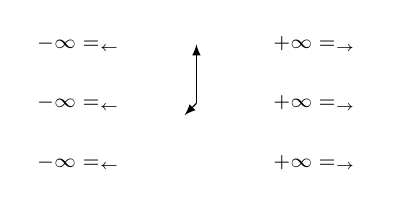
\begin{tikzpicture}[z=.5cm,>=latex,scale=.75,font=\scriptsize]
      \drawcube[draw]
      \begin{scope}[xshift=-3cm,x=3cm]
        \begin{scope}[yshift=-1cm]
          \drawcube[draw,densely dotted]
        \end{scope}
        \begin{scope}
          \drawcube[draw,densely dotted]
        \end{scope}
        \begin{scope}[yshift=1cm]
          \drawcube[draw,densely dotted]
        \end{scope}
      \end{scope}
      \begin{scope}[yshift=-1cm]
        \drawcube[draw,densely dotted]
      \end{scope}
      \begin{scope}[yshift=1cm]
        \drawcube[draw,densely dotted]
      \end{scope}
      \begin{scope}[xshift=1cm,x=3cm]
        \begin{scope}[yshift=-1cm]
          \drawcube[draw,densely dotted]
        \end{scope}
        \begin{scope}
          \drawcube[draw,densely dotted]
        \end{scope}
        \begin{scope}[yshift=1cm]
          \drawcube[draw,densely dotted]
        \end{scope}
      \end{scope}

      % Draw arrows
      \foreach \y in {-.5,.5,1.5} {
          \node[anchor=center] at (-1.5,\y,.5) {$-\infty=\SE_\leftarrow$};
          \node[anchor=center] at (2.5,\y,.5) {$+\infty=\SE_\rightarrow$};
      }
      % \draw[->] (.5,.5,.5) -- (1.5,.5,.5);
      \draw[->] (.5,.5,.5) -- (.5,1.5,.5);
      \draw[->] (.5,.5,.5) -- (.5,.5,.1);

    \end{tikzpicture}

}
      \end{columns}

    \end{center}
    
    \item<4-> Self-energies have ``large'' imaginary components smearing the DOS for states
    coupled to the leads. The imaginary part ($\eta$) can thus often be neglected in the
    device region\footnote<4->{Not for bound states.}.
    
    \end{itemize}

  \end{block}

  
\end{frame}

%%% Local Variables:
%%% mode: latex
%%% TeX-master: "talk"
%%% End:
